\documentclass[twoside]{book}

% Packages required by doxygen
\usepackage{fixltx2e}
\usepackage{calc}
\usepackage{doxygen}
\usepackage[export]{adjustbox} % also loads graphicx
\usepackage{graphicx}
\usepackage[utf8]{inputenc}
\usepackage{makeidx}
\usepackage{multicol}
\usepackage{multirow}
\PassOptionsToPackage{warn}{textcomp}
\usepackage{textcomp}
\usepackage[nointegrals]{wasysym}
\usepackage[table]{xcolor}

% Font selection
\usepackage[T1]{fontenc}
\usepackage[scaled=.90]{helvet}
\usepackage{courier}
\usepackage{amssymb}
\usepackage{sectsty}
\renewcommand{\familydefault}{\sfdefault}
\allsectionsfont{%
  \fontseries{bc}\selectfont%
  \color{darkgray}%
}
\renewcommand{\DoxyLabelFont}{%
  \fontseries{bc}\selectfont%
  \color{darkgray}%
}
\newcommand{\+}{\discretionary{\mbox{\scriptsize$\hookleftarrow$}}{}{}}

% Page & text layout
\usepackage{geometry}
\geometry{%
  a4paper,%
  top=2.5cm,%
  bottom=2.5cm,%
  left=2.5cm,%
  right=2.5cm%
}
\tolerance=750
\hfuzz=15pt
\hbadness=750
\setlength{\emergencystretch}{15pt}
\setlength{\parindent}{0cm}
\setlength{\parskip}{3ex plus 2ex minus 2ex}
\makeatletter
\renewcommand{\paragraph}{%
  \@startsection{paragraph}{4}{0ex}{-1.0ex}{1.0ex}{%
    \normalfont\normalsize\bfseries\SS@parafont%
  }%
}
\renewcommand{\subparagraph}{%
  \@startsection{subparagraph}{5}{0ex}{-1.0ex}{1.0ex}{%
    \normalfont\normalsize\bfseries\SS@subparafont%
  }%
}
\makeatother

% Headers & footers
\usepackage{fancyhdr}
\pagestyle{fancyplain}
\fancyhead[LE]{\fancyplain{}{\bfseries\thepage}}
\fancyhead[CE]{\fancyplain{}{}}
\fancyhead[RE]{\fancyplain{}{\bfseries\leftmark}}
\fancyhead[LO]{\fancyplain{}{\bfseries\rightmark}}
\fancyhead[CO]{\fancyplain{}{}}
\fancyhead[RO]{\fancyplain{}{\bfseries\thepage}}
\fancyfoot[LE]{\fancyplain{}{}}
\fancyfoot[CE]{\fancyplain{}{}}
\fancyfoot[RE]{\fancyplain{}{\bfseries\scriptsize Generated by Doxygen }}
\fancyfoot[LO]{\fancyplain{}{\bfseries\scriptsize Generated by Doxygen }}
\fancyfoot[CO]{\fancyplain{}{}}
\fancyfoot[RO]{\fancyplain{}{}}
\renewcommand{\footrulewidth}{0.4pt}
\renewcommand{\chaptermark}[1]{%
  \markboth{#1}{}%
}
\renewcommand{\sectionmark}[1]{%
  \markright{\thesection\ #1}%
}

% Indices & bibliography
\usepackage{natbib}
\usepackage[titles]{tocloft}
\setcounter{tocdepth}{3}
\setcounter{secnumdepth}{5}
\makeindex

% Hyperlinks (required, but should be loaded last)
\usepackage{ifpdf}
\ifpdf
  \usepackage[pdftex,pagebackref=true]{hyperref}
\else
  \usepackage[ps2pdf,pagebackref=true]{hyperref}
\fi
\hypersetup{%
  colorlinks=true,%
  linkcolor=blue,%
  citecolor=blue,%
  unicode%
}

% Custom commands
\newcommand{\clearemptydoublepage}{%
  \newpage{\pagestyle{empty}\cleardoublepage}%
}

\usepackage{caption}
\captionsetup{labelsep=space,justification=centering,font={bf},singlelinecheck=off,skip=4pt,position=top}

%===== C O N T E N T S =====

\begin{document}

% Titlepage & ToC
\hypersetup{pageanchor=false,
             bookmarksnumbered=true,
             pdfencoding=unicode
            }
\pagenumbering{alph}
\begin{titlepage}
\vspace*{7cm}
\begin{center}%
{\Large Rainbow attack }\\
\vspace*{1cm}
{\large Generated by Doxygen 1.8.13}\\
\end{center}
\end{titlepage}
\clearemptydoublepage
\pagenumbering{roman}
\tableofcontents
\clearemptydoublepage
\pagenumbering{arabic}
\hypersetup{pageanchor=true}

%--- Begin generated contents ---
\chapter{Rainbow attack}
\label{index}\hypertarget{index}{}\subsection*{Goal}

The objective of this homework is to implement an attack on password tables with a rainbow table.

\subsection*{Structure}

Build files are in folder {\ttfamily build}.

Source files are in folder {\ttfamily src}. You can find 3 subfolders, one to \hyperlink{namespacebe_1_1esi_1_1secl_1_1pn_af8b773cad93b0eb78b89f69721e4bb1d}{generate the Rainbow Table}, one to do the \hyperlink{namespacebe_1_1esi_1_1secl_1_1pn_aad832fb30fa4cc9e74d15d7129d0c929}{Rainbow Attack}, and some utils.

{\ttfamily rsc} will contain the rainbow table, the cracked passwords and the cracked passwords hashes.

\subsection*{How to}

To set up the project and launch it with default values, use command {\ttfamily make}. It will \+:
\begin{DoxyItemize}
\item install or update {\ttfamily sqlite}, {\ttfamily libsqlite3-\/dev}, {\ttfamily gcc-\/8} and {\ttfamily g++-\/8},
\item build the project,
\item launch the project (generate the RT and crack some hashes).
\end{DoxyItemize}

To set up the project and launch it \+:
\begin{DoxyItemize}
\item install or update sqlite and gcc/g++ (wich are require) with command {\ttfamily make setup},
\item build the project with command {\ttfamily make build}.
\item generate the rainbow table with command {\ttfamily build/generate\+RT number\+Of\+Head number\+Of\+Reduce},
\item generate the rainbow table with command {\ttfamily build/crack\+RT}.
\end{DoxyItemize}

\subsection*{Know bugs}

None.

\subsection*{Authors}

43197 Patti Philippe.

43121 Baltofski Nicolas. 
\chapter{Namespace Index}
\section{Namespace List}
Here is a list of all namespaces with brief descriptions\+:\begin{DoxyCompactList}
\item\contentsline{section}{\hyperlink{namespacebe}{be} }{\pageref{namespacebe}}{}
\item\contentsline{section}{\hyperlink{namespacebe_1_1esi}{be\+::esi} }{\pageref{namespacebe_1_1esi}}{}
\item\contentsline{section}{\hyperlink{namespacebe_1_1esi_1_1secl}{be\+::esi\+::secl} }{\pageref{namespacebe_1_1esi_1_1secl}}{}
\item\contentsline{section}{\hyperlink{namespacebe_1_1esi_1_1secl_1_1pn}{be\+::esi\+::secl\+::pn} }{\pageref{namespacebe_1_1esi_1_1secl_1_1pn}}{}
\end{DoxyCompactList}

\chapter{File Index}
\section{File List}
Here is a list of all files with brief descriptions\+:\begin{DoxyCompactList}
\item\contentsline{section}{src/crack/\hyperlink{crackRT_8cpp}{crack\+R\+T.\+cpp} \\*Declaration of functions of \hyperlink{crackRT_8h}{crack\+R\+T.\+h} }{\pageref{crackRT_8cpp}}{}
\item\contentsline{section}{src/crack/\hyperlink{crackRT_8h}{crack\+R\+T.\+h} \\*Declaration of functions of \hyperlink{crackRT_8h}{crack\+R\+T.\+h} }{\pageref{crackRT_8h}}{}
\item\contentsline{section}{src/crack/\hyperlink{crack_2main_8cpp}{main.\+cpp} }{\pageref{crack_2main_8cpp}}{}
\item\contentsline{section}{src/generate\+R\+T/\hyperlink{generateRT_8cpp}{generate\+R\+T.\+cpp} \\*Definition of function of \hyperlink{generateRT_8h}{generate\+R\+T.\+h} }{\pageref{generateRT_8cpp}}{}
\item\contentsline{section}{src/generate\+R\+T/\hyperlink{generateRT_8h}{generate\+R\+T.\+h} \\*Declaration of functions for \hyperlink{generateRT_8cpp}{generate\+R\+T.\+cpp} }{\pageref{generateRT_8h}}{}
\item\contentsline{section}{src/generate\+R\+T/\hyperlink{generateRT_2main_8cpp}{main.\+cpp} }{\pageref{generateRT_2main_8cpp}}{}
\end{DoxyCompactList}

\chapter{Namespace Documentation}
\hypertarget{namespacebe}{}\section{be Namespace Reference}
\label{namespacebe}\index{be@{be}}
\subsection*{Namespaces}
\begin{DoxyCompactItemize}
\item 
 \hyperlink{namespacebe_1_1esi}{esi}
\end{DoxyCompactItemize}

\hypertarget{namespacebe_1_1esi}{}\section{be\+:\+:esi Namespace Reference}
\label{namespacebe_1_1esi}\index{be\+::esi@{be\+::esi}}
\subsection*{Namespaces}
\begin{DoxyCompactItemize}
\item 
 \hyperlink{namespacebe_1_1esi_1_1secl}{secl}
\end{DoxyCompactItemize}

\hypertarget{namespacebe_1_1esi_1_1secl}{}\section{be\+:\+:esi\+:\+:secl Namespace Reference}
\label{namespacebe_1_1esi_1_1secl}\index{be\+::esi\+::secl@{be\+::esi\+::secl}}
\subsection*{Namespaces}
\begin{DoxyCompactItemize}
\item 
 \hyperlink{namespacebe_1_1esi_1_1secl_1_1pn}{pn}
\end{DoxyCompactItemize}

\hypertarget{namespacebe_1_1esi_1_1secl_1_1pn}{}\section{be\+:\+:esi\+:\+:secl\+:\+:pn Namespace Reference}
\label{namespacebe_1_1esi_1_1secl_1_1pn}\index{be\+::esi\+::secl\+::pn@{be\+::esi\+::secl\+::pn}}
\subsection*{Functions}
\begin{DoxyCompactItemize}
\item 
void \hyperlink{namespacebe_1_1esi_1_1secl_1_1pn_aad832fb30fa4cc9e74d15d7129d0c929}{crack} (const std\+::string \&hash\+File, sqlite3 $\ast$db, const std\+::string \&cracked\+Pwd\+File, const std\+::string \&cracked\+Hash\+File)
\begin{DoxyCompactList}\small\item\em Attempts to find passwords corresponding to the hashes given, at the hand of the tails. \end{DoxyCompactList}\item 
void \hyperlink{namespacebe_1_1esi_1_1secl_1_1pn_a5421a253f4c247695a0f26055ecc4dea}{crack\+In\+Thread} (std\+::ifstream \&hashes\+Input, sqlite3 $\ast$db, std\+::ofstream \&cracked\+Pwd\+Output, std\+::ofstream \&cracked\+Hash\+Output)
\begin{DoxyCompactList}\small\item\em Crack function to call with a thread. \end{DoxyCompactList}\item 
std\+::string \hyperlink{namespacebe_1_1esi_1_1secl_1_1pn_a44dea6059d3689561497f5f03e09dac2}{get\+Tail} (const std\+::string \&hash, sqlite3\+\_\+stmt $\ast$stmt\+Read\+Tail, int \&idx\+Reduction)
\begin{DoxyCompactList}\small\item\em Searches the tail of the hash and return it. \end{DoxyCompactList}\item 
std\+::string \hyperlink{namespacebe_1_1esi_1_1secl_1_1pn_a4f2bdcedf26f904e1e07776955d80d97}{get\+Head} (sqlite3\+\_\+stmt $\ast$stmt\+Get\+Head, std\+::string tail)
\begin{DoxyCompactList}\small\item\em Get the head of a tail. \end{DoxyCompactList}\item 
std\+::string \hyperlink{namespacebe_1_1esi_1_1secl_1_1pn_ae68f13fff76cabc930b60594c300a168}{find\+Pwd} (std\+::string head, int idx\+Reduction)
\begin{DoxyCompactList}\small\item\em Computes the password after idx\+Reduction reductions. \end{DoxyCompactList}\item 
void \hyperlink{namespacebe_1_1esi_1_1secl_1_1pn_af8b773cad93b0eb78b89f69721e4bb1d}{generate\+RT} (sqlite3 $\ast$db, unsigned nb\+Head=\hyperlink{namespacebe_1_1esi_1_1secl_1_1pn_a3f7aaccb1bf4e47f92d72bf9b2471328}{N\+B\+\_\+\+H\+E\+AD}, int nb\+Reduce=\hyperlink{namespacebe_1_1esi_1_1secl_1_1pn_a9434f9e96778e243fcb677633df38598}{N\+B\+\_\+\+R\+E\+D\+U\+CE})
\begin{DoxyCompactList}\small\item\em Generate the head and the tails of the RT, and write them into the DB. \end{DoxyCompactList}\item 
void \hyperlink{namespacebe_1_1esi_1_1secl_1_1pn_aaf5216f5718720c15b5925f7e8a94d10}{generate\+R\+T\+In\+Thread} (sqlite3 $\ast$db, unsigned nb\+Head, int nb\+Reduce)
\begin{DoxyCompactList}\small\item\em Generate the head and the tails of the RT, and write them into the DB. \end{DoxyCompactList}\item 
const std\+::string \hyperlink{namespacebe_1_1esi_1_1secl_1_1pn_a6b6903f68a7fbdcd8e705dc2b9c28c03}{D\+B\+\_\+\+N\+A\+ME} (\char`\"{}rsc/rt\+\_\+6\+\_\+2\+\_\+1000000\+\_\+1000.\+sqlite\char`\"{})
\begin{DoxyCompactList}\small\item\em The relative path to the DB. \end{DoxyCompactList}\end{DoxyCompactItemize}
\subsection*{Variables}
\begin{DoxyCompactItemize}
\item 
std\+::mutex \hyperlink{namespacebe_1_1esi_1_1secl_1_1pn_ad1391e7f8a94f1b945665f76d1965070}{mtx\+Read\+Head}
\begin{DoxyCompactList}\small\item\em Mutex to read the head file with concurency. \end{DoxyCompactList}\item 
std\+::mutex \hyperlink{namespacebe_1_1esi_1_1secl_1_1pn_a11fbbf54ca476439788d44d4d50512ab}{mtx\+Print\+Cracked}
\begin{DoxyCompactList}\small\item\em Mutex to write cracked password and hashes with concurency. \end{DoxyCompactList}\item 
const unsigned \hyperlink{namespacebe_1_1esi_1_1secl_1_1pn_a0bd77d0531142c20d01ec002cd3c210a}{N\+B\+\_\+\+T\+H\+R\+E\+A\+DS} = 10
\begin{DoxyCompactList}\small\item\em How many threads to run to crack. \end{DoxyCompactList}\item 
const char $\ast$ \hyperlink{namespacebe_1_1esi_1_1secl_1_1pn_a878205e4dbef8040fb12f6afb8717fa9}{S\+E\+L\+E\+C\+T\+\_\+\+T\+A\+IL} = \char`\"{}S\+E\+L\+E\+CT tail F\+R\+OM R\+A\+I\+N\+B\+O\+W\+\_\+\+T\+A\+B\+LE W\+H\+E\+RE tail = ?;\char`\"{}
\begin{DoxyCompactList}\small\item\em Select a tail. \end{DoxyCompactList}\item 
const char $\ast$ \hyperlink{namespacebe_1_1esi_1_1secl_1_1pn_a90db4018123c098c9cd9205b69c1d2e5}{S\+E\+L\+E\+C\+T\+\_\+\+H\+E\+AD} = \char`\"{}S\+E\+L\+E\+CT head F\+R\+OM R\+A\+I\+N\+B\+O\+W\+\_\+\+T\+A\+B\+LE W\+H\+E\+RE tail = ?;\char`\"{}
\begin{DoxyCompactList}\small\item\em Select the head of the tail. \end{DoxyCompactList}\item 
const unsigned \hyperlink{namespacebe_1_1esi_1_1secl_1_1pn_a6b1322df9a3137fe3dff27602a0dd390}{N\+B\+\_\+\+T\+H\+R\+E\+A\+D\+S\+\_\+\+G\+E\+N\+E\+R\+A\+TE} = 10
\begin{DoxyCompactList}\small\item\em Number of thread to create to generate the RT. \end{DoxyCompactList}\item 
const unsigned \hyperlink{namespacebe_1_1esi_1_1secl_1_1pn_a3f7aaccb1bf4e47f92d72bf9b2471328}{N\+B\+\_\+\+H\+E\+AD} = 500000000
\begin{DoxyCompactList}\small\item\em How many password we generate for the RT. \end{DoxyCompactList}\item 
const int \hyperlink{namespacebe_1_1esi_1_1secl_1_1pn_a9434f9e96778e243fcb677633df38598}{N\+B\+\_\+\+R\+E\+D\+U\+CE} = 160
\begin{DoxyCompactList}\small\item\em How many reduce function we use before getting the tail. \end{DoxyCompactList}\item 
const unsigned \hyperlink{namespacebe_1_1esi_1_1secl_1_1pn_ac4d6305d2a5baed196042f8a30533620}{M\+I\+N\+\_\+\+P\+W\+D\+\_\+\+S\+I\+ZE} = 6
\begin{DoxyCompactList}\small\item\em The minimal password size. \end{DoxyCompactList}\item 
const unsigned \hyperlink{namespacebe_1_1esi_1_1secl_1_1pn_a2e3241ac36dabdb668b68028e097dded}{M\+A\+X\+\_\+\+P\+W\+D\+\_\+\+S\+I\+ZE} = 6
\begin{DoxyCompactList}\small\item\em The maximal password size. \end{DoxyCompactList}\item 
const char $\ast$ \hyperlink{namespacebe_1_1esi_1_1secl_1_1pn_a6dae14cb83aa871e50c9aaea7f776055}{D\+R\+O\+P\+\_\+\+RT} = \char`\"{}D\+R\+OP T\+A\+B\+LE IF E\+X\+I\+S\+TS R\+A\+I\+N\+B\+O\+W\+\_\+\+T\+A\+B\+LE;\char`\"{}
\item 
const char $\ast$ \hyperlink{namespacebe_1_1esi_1_1secl_1_1pn_ab39f379fcf2d9342096df70dcf998d32}{C\+R\+E\+A\+T\+E\+\_\+\+RT} = \char`\"{}C\+R\+E\+A\+TE T\+A\+B\+LE R\+A\+I\+N\+B\+O\+W\+\_\+\+T\+A\+B\+LE (head C\+H\+AR(8) P\+R\+I\+M\+A\+RY K\+EY, tail C\+H\+AR(8) N\+OT N\+U\+LL U\+N\+I\+Q\+UE);\char`\"{}
\item 
const char $\ast$ \hyperlink{namespacebe_1_1esi_1_1secl_1_1pn_a93b0970fb08c37d478307bfadfb3b775}{I\+N\+S\+E\+R\+T\+\_\+\+RT} = \char`\"{}I\+N\+S\+E\+RT OR I\+G\+N\+O\+RE I\+N\+TO R\+A\+I\+N\+B\+O\+W\+\_\+\+T\+A\+B\+LE (head, tail) V\+A\+L\+U\+ES (?, ?);\char`\"{}
\end{DoxyCompactItemize}


\subsection{Function Documentation}
\mbox{\Hypertarget{namespacebe_1_1esi_1_1secl_1_1pn_aad832fb30fa4cc9e74d15d7129d0c929}\label{namespacebe_1_1esi_1_1secl_1_1pn_aad832fb30fa4cc9e74d15d7129d0c929}} 
\index{be\+::esi\+::secl\+::pn@{be\+::esi\+::secl\+::pn}!crack@{crack}}
\index{crack@{crack}!be\+::esi\+::secl\+::pn@{be\+::esi\+::secl\+::pn}}
\subsubsection{\texorpdfstring{crack()}{crack()}}
{\footnotesize\ttfamily void be\+::esi\+::secl\+::pn\+::crack (\begin{DoxyParamCaption}\item[{const std\+::string \&}]{hash\+File,  }\item[{sqlite3 $\ast$}]{db,  }\item[{const std\+::string \&}]{cracked\+Pwd\+File,  }\item[{const std\+::string \&}]{cracked\+Hash\+File }\end{DoxyParamCaption})}



Attempts to find passwords corresponding to the hashes given, at the hand of the tails. 

Using a opened sqlite rainbow table, should have been created with generate\+RT to have a good structure. Crack is performed in multiple threads. 
\begin{DoxyParams}{Parameters}
{\em hash\+File} & The file\textquotesingle{}s name containing the hashes to crack. \\
\hline
{\em db} & The db containing the rainbow table. \\
\hline
{\em cracked\+Pwd\+File} & The file\textquotesingle{}s name for the cracked passwords. \\
\hline
{\em cracked\+Hash\+File} & The file\textquotesingle{}s name for the hashes of the cracked passwords. Each line is the hash of the password of the same line of the passwords file. \\
\hline
\end{DoxyParams}

\begin{DoxyExceptions}{Exceptions}
{\em std\+::runtime\+\_\+error} & if hash\+File, head\+File, tails\+File or cracked\+File can\textquotesingle{}t be opened. \\
\hline
\end{DoxyExceptions}
\mbox{\Hypertarget{namespacebe_1_1esi_1_1secl_1_1pn_a5421a253f4c247695a0f26055ecc4dea}\label{namespacebe_1_1esi_1_1secl_1_1pn_a5421a253f4c247695a0f26055ecc4dea}} 
\index{be\+::esi\+::secl\+::pn@{be\+::esi\+::secl\+::pn}!crack\+In\+Thread@{crack\+In\+Thread}}
\index{crack\+In\+Thread@{crack\+In\+Thread}!be\+::esi\+::secl\+::pn@{be\+::esi\+::secl\+::pn}}
\subsubsection{\texorpdfstring{crack\+In\+Thread()}{crackInThread()}}
{\footnotesize\ttfamily void be\+::esi\+::secl\+::pn\+::crack\+In\+Thread (\begin{DoxyParamCaption}\item[{std\+::ifstream \&}]{hashes\+Input,  }\item[{sqlite3 $\ast$}]{db,  }\item[{std\+::ofstream \&}]{cracked\+Pwd\+Output,  }\item[{std\+::ofstream \&}]{cracked\+Hash\+Output }\end{DoxyParamCaption})}



Crack function to call with a thread. 

Read and write with file is performed with mutex. 
\begin{DoxyParams}{Parameters}
{\em hashed\+Input} & The hashes file. \\
\hline
{\em db} & The DB. \\
\hline
{\em cracked\+Pwd\+Output} & The file\textquotesingle{}s name for the cracked passwords. \\
\hline
{\em cracked\+Hash\+Output} & The file\textquotesingle{}s name for the hashes of the cracked passwords. Each line is the hash of the password of the same line of the passwords file. \\
\hline
\end{DoxyParams}
\mbox{\Hypertarget{namespacebe_1_1esi_1_1secl_1_1pn_a6b6903f68a7fbdcd8e705dc2b9c28c03}\label{namespacebe_1_1esi_1_1secl_1_1pn_a6b6903f68a7fbdcd8e705dc2b9c28c03}} 
\index{be\+::esi\+::secl\+::pn@{be\+::esi\+::secl\+::pn}!D\+B\+\_\+\+N\+A\+ME@{D\+B\+\_\+\+N\+A\+ME}}
\index{D\+B\+\_\+\+N\+A\+ME@{D\+B\+\_\+\+N\+A\+ME}!be\+::esi\+::secl\+::pn@{be\+::esi\+::secl\+::pn}}
\subsubsection{\texorpdfstring{D\+B\+\_\+\+N\+A\+M\+E()}{DB\_NAME()}}
{\footnotesize\ttfamily const std\+::string be\+::esi\+::secl\+::pn\+::\+D\+B\+\_\+\+N\+A\+ME (\begin{DoxyParamCaption}\item[{\char`\"{}rsc/rt\+\_\+6\+\_\+2\+\_\+1000000\+\_\+1000.\+sqlite\char`\"{}}]{ }\end{DoxyParamCaption})\hspace{0.3cm}{\ttfamily [inline]}}



The relative path to the DB. 

\mbox{\Hypertarget{namespacebe_1_1esi_1_1secl_1_1pn_ae68f13fff76cabc930b60594c300a168}\label{namespacebe_1_1esi_1_1secl_1_1pn_ae68f13fff76cabc930b60594c300a168}} 
\index{be\+::esi\+::secl\+::pn@{be\+::esi\+::secl\+::pn}!find\+Pwd@{find\+Pwd}}
\index{find\+Pwd@{find\+Pwd}!be\+::esi\+::secl\+::pn@{be\+::esi\+::secl\+::pn}}
\subsubsection{\texorpdfstring{find\+Pwd()}{findPwd()}}
{\footnotesize\ttfamily std\+::string be\+::esi\+::secl\+::pn\+::find\+Pwd (\begin{DoxyParamCaption}\item[{std\+::string}]{head,  }\item[{int}]{idx\+Reduction }\end{DoxyParamCaption})}



Computes the password after idx\+Reduction reductions. 


\begin{DoxyParams}{Parameters}
{\em head} & The head of the line. \\
\hline
{\em idx\+Reduction} & The number of reductions to perform. \\
\hline
\end{DoxyParams}
\begin{DoxyReturn}{Returns}
The found password. 
\end{DoxyReturn}
\mbox{\Hypertarget{namespacebe_1_1esi_1_1secl_1_1pn_af8b773cad93b0eb78b89f69721e4bb1d}\label{namespacebe_1_1esi_1_1secl_1_1pn_af8b773cad93b0eb78b89f69721e4bb1d}} 
\index{be\+::esi\+::secl\+::pn@{be\+::esi\+::secl\+::pn}!generate\+RT@{generate\+RT}}
\index{generate\+RT@{generate\+RT}!be\+::esi\+::secl\+::pn@{be\+::esi\+::secl\+::pn}}
\subsubsection{\texorpdfstring{generate\+R\+T()}{generateRT()}}
{\footnotesize\ttfamily void be\+::esi\+::secl\+::pn\+::generate\+RT (\begin{DoxyParamCaption}\item[{sqlite3 $\ast$}]{db,  }\item[{unsigned}]{nb\+Head = {\ttfamily \hyperlink{namespacebe_1_1esi_1_1secl_1_1pn_a3f7aaccb1bf4e47f92d72bf9b2471328}{N\+B\+\_\+\+H\+E\+AD}},  }\item[{int}]{nb\+Reduce = {\ttfamily \hyperlink{namespacebe_1_1esi_1_1secl_1_1pn_a9434f9e96778e243fcb677633df38598}{N\+B\+\_\+\+R\+E\+D\+U\+CE}} }\end{DoxyParamCaption})}



Generate the head and the tails of the RT, and write them into the DB. 

The tails are computed after a number of reductions, based on their hash. Drop the table if exists. 
\begin{DoxyParams}{Parameters}
{\em db} & The db to store the passwords and the tails. It must be a valid db. \\
\hline
{\em nb\+Head} & The number of head to generate. \\
\hline
{\em nb\+Reduce} & The number of reduction functions to apply to compute the tail. If not set, use default value. \\
\hline
\end{DoxyParams}
\mbox{\Hypertarget{namespacebe_1_1esi_1_1secl_1_1pn_aaf5216f5718720c15b5925f7e8a94d10}\label{namespacebe_1_1esi_1_1secl_1_1pn_aaf5216f5718720c15b5925f7e8a94d10}} 
\index{be\+::esi\+::secl\+::pn@{be\+::esi\+::secl\+::pn}!generate\+R\+T\+In\+Thread@{generate\+R\+T\+In\+Thread}}
\index{generate\+R\+T\+In\+Thread@{generate\+R\+T\+In\+Thread}!be\+::esi\+::secl\+::pn@{be\+::esi\+::secl\+::pn}}
\subsubsection{\texorpdfstring{generate\+R\+T\+In\+Thread()}{generateRTInThread()}}
{\footnotesize\ttfamily void be\+::esi\+::secl\+::pn\+::generate\+R\+T\+In\+Thread (\begin{DoxyParamCaption}\item[{sqlite3 $\ast$}]{db,  }\item[{unsigned}]{nb\+Head,  }\item[{int}]{nb\+Reduce }\end{DoxyParamCaption})}



Generate the head and the tails of the RT, and write them into the DB. 

This function is for thread. The tails are computed after a number of reductions, based on their hash. 
\begin{DoxyParams}{Parameters}
{\em db} & The db to store the passwords and the tails. It must be a valid db. \\
\hline
{\em nb\+Head} & The number of head to generate. \\
\hline
{\em nb\+Reduce} & The number of reduction functions to apply to compute the tail. If not set, use default value. \\
\hline
\end{DoxyParams}
\mbox{\Hypertarget{namespacebe_1_1esi_1_1secl_1_1pn_a4f2bdcedf26f904e1e07776955d80d97}\label{namespacebe_1_1esi_1_1secl_1_1pn_a4f2bdcedf26f904e1e07776955d80d97}} 
\index{be\+::esi\+::secl\+::pn@{be\+::esi\+::secl\+::pn}!get\+Head@{get\+Head}}
\index{get\+Head@{get\+Head}!be\+::esi\+::secl\+::pn@{be\+::esi\+::secl\+::pn}}
\subsubsection{\texorpdfstring{get\+Head()}{getHead()}}
{\footnotesize\ttfamily std\+::string be\+::esi\+::secl\+::pn\+::get\+Head (\begin{DoxyParamCaption}\item[{sqlite3\+\_\+stmt $\ast$}]{stmt\+Get\+Head,  }\item[{std\+::string}]{tail }\end{DoxyParamCaption})}



Get the head of a tail. 


\begin{DoxyParams}{Parameters}
{\em stmt\+Get\+Head} & The statement to apply. \\
\hline
{\em tail} & The tail of the search head \\
\hline
\end{DoxyParams}
\begin{DoxyReturn}{Returns}
the head of the tail 
\end{DoxyReturn}

\begin{DoxyExceptions}{Exceptions}
{\em std\+::runtime\+\_\+error} & if no tail found \\
\hline
\end{DoxyExceptions}
\mbox{\Hypertarget{namespacebe_1_1esi_1_1secl_1_1pn_a44dea6059d3689561497f5f03e09dac2}\label{namespacebe_1_1esi_1_1secl_1_1pn_a44dea6059d3689561497f5f03e09dac2}} 
\index{be\+::esi\+::secl\+::pn@{be\+::esi\+::secl\+::pn}!get\+Tail@{get\+Tail}}
\index{get\+Tail@{get\+Tail}!be\+::esi\+::secl\+::pn@{be\+::esi\+::secl\+::pn}}
\subsubsection{\texorpdfstring{get\+Tail()}{getTail()}}
{\footnotesize\ttfamily std\+::string be\+::esi\+::secl\+::pn\+::get\+Tail (\begin{DoxyParamCaption}\item[{const std\+::string \&}]{hash,  }\item[{sqlite3\+\_\+stmt $\ast$}]{stmt\+Read\+Tail,  }\item[{int \&}]{idx\+Reduction }\end{DoxyParamCaption})}



Searches the tail of the hash and return it. 

Otherwise, return an empty string 
\begin{DoxyParams}{Parameters}
{\em hash} & The src hash to find. \\
\hline
{\em stmt\+Read\+Tail} & The prepared statement to search a tail in the database. \\
\hline
{\em idx\+Reduction} & The number of reductions performed to find the hash. \\
\hline
\end{DoxyParams}
\begin{DoxyReturn}{Returns}
The tail of the hash, or an empty string if no tail is found. 
\end{DoxyReturn}


\subsection{Variable Documentation}
\mbox{\Hypertarget{namespacebe_1_1esi_1_1secl_1_1pn_ab39f379fcf2d9342096df70dcf998d32}\label{namespacebe_1_1esi_1_1secl_1_1pn_ab39f379fcf2d9342096df70dcf998d32}} 
\index{be\+::esi\+::secl\+::pn@{be\+::esi\+::secl\+::pn}!C\+R\+E\+A\+T\+E\+\_\+\+RT@{C\+R\+E\+A\+T\+E\+\_\+\+RT}}
\index{C\+R\+E\+A\+T\+E\+\_\+\+RT@{C\+R\+E\+A\+T\+E\+\_\+\+RT}!be\+::esi\+::secl\+::pn@{be\+::esi\+::secl\+::pn}}
\subsubsection{\texorpdfstring{C\+R\+E\+A\+T\+E\+\_\+\+RT}{CREATE\_RT}}
{\footnotesize\ttfamily const char$\ast$ be\+::esi\+::secl\+::pn\+::\+C\+R\+E\+A\+T\+E\+\_\+\+RT = \char`\"{}C\+R\+E\+A\+TE T\+A\+B\+LE R\+A\+I\+N\+B\+O\+W\+\_\+\+T\+A\+B\+LE (head C\+H\+AR(8) P\+R\+I\+M\+A\+RY K\+EY, tail C\+H\+AR(8) N\+OT N\+U\+LL U\+N\+I\+Q\+UE);\char`\"{}\hspace{0.3cm}{\ttfamily [inline]}}

\mbox{\Hypertarget{namespacebe_1_1esi_1_1secl_1_1pn_a6dae14cb83aa871e50c9aaea7f776055}\label{namespacebe_1_1esi_1_1secl_1_1pn_a6dae14cb83aa871e50c9aaea7f776055}} 
\index{be\+::esi\+::secl\+::pn@{be\+::esi\+::secl\+::pn}!D\+R\+O\+P\+\_\+\+RT@{D\+R\+O\+P\+\_\+\+RT}}
\index{D\+R\+O\+P\+\_\+\+RT@{D\+R\+O\+P\+\_\+\+RT}!be\+::esi\+::secl\+::pn@{be\+::esi\+::secl\+::pn}}
\subsubsection{\texorpdfstring{D\+R\+O\+P\+\_\+\+RT}{DROP\_RT}}
{\footnotesize\ttfamily const char$\ast$ be\+::esi\+::secl\+::pn\+::\+D\+R\+O\+P\+\_\+\+RT = \char`\"{}D\+R\+OP T\+A\+B\+LE IF E\+X\+I\+S\+TS R\+A\+I\+N\+B\+O\+W\+\_\+\+T\+A\+B\+LE;\char`\"{}\hspace{0.3cm}{\ttfamily [inline]}}

\mbox{\Hypertarget{namespacebe_1_1esi_1_1secl_1_1pn_a93b0970fb08c37d478307bfadfb3b775}\label{namespacebe_1_1esi_1_1secl_1_1pn_a93b0970fb08c37d478307bfadfb3b775}} 
\index{be\+::esi\+::secl\+::pn@{be\+::esi\+::secl\+::pn}!I\+N\+S\+E\+R\+T\+\_\+\+RT@{I\+N\+S\+E\+R\+T\+\_\+\+RT}}
\index{I\+N\+S\+E\+R\+T\+\_\+\+RT@{I\+N\+S\+E\+R\+T\+\_\+\+RT}!be\+::esi\+::secl\+::pn@{be\+::esi\+::secl\+::pn}}
\subsubsection{\texorpdfstring{I\+N\+S\+E\+R\+T\+\_\+\+RT}{INSERT\_RT}}
{\footnotesize\ttfamily const char$\ast$ be\+::esi\+::secl\+::pn\+::\+I\+N\+S\+E\+R\+T\+\_\+\+RT = \char`\"{}I\+N\+S\+E\+RT OR I\+G\+N\+O\+RE I\+N\+TO R\+A\+I\+N\+B\+O\+W\+\_\+\+T\+A\+B\+LE (head, tail) V\+A\+L\+U\+ES (?, ?);\char`\"{}\hspace{0.3cm}{\ttfamily [inline]}}

\mbox{\Hypertarget{namespacebe_1_1esi_1_1secl_1_1pn_a2e3241ac36dabdb668b68028e097dded}\label{namespacebe_1_1esi_1_1secl_1_1pn_a2e3241ac36dabdb668b68028e097dded}} 
\index{be\+::esi\+::secl\+::pn@{be\+::esi\+::secl\+::pn}!M\+A\+X\+\_\+\+P\+W\+D\+\_\+\+S\+I\+ZE@{M\+A\+X\+\_\+\+P\+W\+D\+\_\+\+S\+I\+ZE}}
\index{M\+A\+X\+\_\+\+P\+W\+D\+\_\+\+S\+I\+ZE@{M\+A\+X\+\_\+\+P\+W\+D\+\_\+\+S\+I\+ZE}!be\+::esi\+::secl\+::pn@{be\+::esi\+::secl\+::pn}}
\subsubsection{\texorpdfstring{M\+A\+X\+\_\+\+P\+W\+D\+\_\+\+S\+I\+ZE}{MAX\_PWD\_SIZE}}
{\footnotesize\ttfamily const unsigned be\+::esi\+::secl\+::pn\+::\+M\+A\+X\+\_\+\+P\+W\+D\+\_\+\+S\+I\+ZE = 6\hspace{0.3cm}{\ttfamily [inline]}}



The maximal password size. 

\mbox{\Hypertarget{namespacebe_1_1esi_1_1secl_1_1pn_ac4d6305d2a5baed196042f8a30533620}\label{namespacebe_1_1esi_1_1secl_1_1pn_ac4d6305d2a5baed196042f8a30533620}} 
\index{be\+::esi\+::secl\+::pn@{be\+::esi\+::secl\+::pn}!M\+I\+N\+\_\+\+P\+W\+D\+\_\+\+S\+I\+ZE@{M\+I\+N\+\_\+\+P\+W\+D\+\_\+\+S\+I\+ZE}}
\index{M\+I\+N\+\_\+\+P\+W\+D\+\_\+\+S\+I\+ZE@{M\+I\+N\+\_\+\+P\+W\+D\+\_\+\+S\+I\+ZE}!be\+::esi\+::secl\+::pn@{be\+::esi\+::secl\+::pn}}
\subsubsection{\texorpdfstring{M\+I\+N\+\_\+\+P\+W\+D\+\_\+\+S\+I\+ZE}{MIN\_PWD\_SIZE}}
{\footnotesize\ttfamily const unsigned be\+::esi\+::secl\+::pn\+::\+M\+I\+N\+\_\+\+P\+W\+D\+\_\+\+S\+I\+ZE = 6\hspace{0.3cm}{\ttfamily [inline]}}



The minimal password size. 

\mbox{\Hypertarget{namespacebe_1_1esi_1_1secl_1_1pn_a11fbbf54ca476439788d44d4d50512ab}\label{namespacebe_1_1esi_1_1secl_1_1pn_a11fbbf54ca476439788d44d4d50512ab}} 
\index{be\+::esi\+::secl\+::pn@{be\+::esi\+::secl\+::pn}!mtx\+Print\+Cracked@{mtx\+Print\+Cracked}}
\index{mtx\+Print\+Cracked@{mtx\+Print\+Cracked}!be\+::esi\+::secl\+::pn@{be\+::esi\+::secl\+::pn}}
\subsubsection{\texorpdfstring{mtx\+Print\+Cracked}{mtxPrintCracked}}
{\footnotesize\ttfamily std\+::mutex be\+::esi\+::secl\+::pn\+::mtx\+Print\+Cracked}



Mutex to write cracked password and hashes with concurency. 

\mbox{\Hypertarget{namespacebe_1_1esi_1_1secl_1_1pn_ad1391e7f8a94f1b945665f76d1965070}\label{namespacebe_1_1esi_1_1secl_1_1pn_ad1391e7f8a94f1b945665f76d1965070}} 
\index{be\+::esi\+::secl\+::pn@{be\+::esi\+::secl\+::pn}!mtx\+Read\+Head@{mtx\+Read\+Head}}
\index{mtx\+Read\+Head@{mtx\+Read\+Head}!be\+::esi\+::secl\+::pn@{be\+::esi\+::secl\+::pn}}
\subsubsection{\texorpdfstring{mtx\+Read\+Head}{mtxReadHead}}
{\footnotesize\ttfamily std\+::mutex be\+::esi\+::secl\+::pn\+::mtx\+Read\+Head}



Mutex to read the head file with concurency. 

\mbox{\Hypertarget{namespacebe_1_1esi_1_1secl_1_1pn_a3f7aaccb1bf4e47f92d72bf9b2471328}\label{namespacebe_1_1esi_1_1secl_1_1pn_a3f7aaccb1bf4e47f92d72bf9b2471328}} 
\index{be\+::esi\+::secl\+::pn@{be\+::esi\+::secl\+::pn}!N\+B\+\_\+\+H\+E\+AD@{N\+B\+\_\+\+H\+E\+AD}}
\index{N\+B\+\_\+\+H\+E\+AD@{N\+B\+\_\+\+H\+E\+AD}!be\+::esi\+::secl\+::pn@{be\+::esi\+::secl\+::pn}}
\subsubsection{\texorpdfstring{N\+B\+\_\+\+H\+E\+AD}{NB\_HEAD}}
{\footnotesize\ttfamily const unsigned be\+::esi\+::secl\+::pn\+::\+N\+B\+\_\+\+H\+E\+AD = 500000000\hspace{0.3cm}{\ttfamily [inline]}}



How many password we generate for the RT. 

\mbox{\Hypertarget{namespacebe_1_1esi_1_1secl_1_1pn_a9434f9e96778e243fcb677633df38598}\label{namespacebe_1_1esi_1_1secl_1_1pn_a9434f9e96778e243fcb677633df38598}} 
\index{be\+::esi\+::secl\+::pn@{be\+::esi\+::secl\+::pn}!N\+B\+\_\+\+R\+E\+D\+U\+CE@{N\+B\+\_\+\+R\+E\+D\+U\+CE}}
\index{N\+B\+\_\+\+R\+E\+D\+U\+CE@{N\+B\+\_\+\+R\+E\+D\+U\+CE}!be\+::esi\+::secl\+::pn@{be\+::esi\+::secl\+::pn}}
\subsubsection{\texorpdfstring{N\+B\+\_\+\+R\+E\+D\+U\+CE}{NB\_REDUCE}}
{\footnotesize\ttfamily const int be\+::esi\+::secl\+::pn\+::\+N\+B\+\_\+\+R\+E\+D\+U\+CE = 160\hspace{0.3cm}{\ttfamily [inline]}}



How many reduce function we use before getting the tail. 

\mbox{\Hypertarget{namespacebe_1_1esi_1_1secl_1_1pn_a0bd77d0531142c20d01ec002cd3c210a}\label{namespacebe_1_1esi_1_1secl_1_1pn_a0bd77d0531142c20d01ec002cd3c210a}} 
\index{be\+::esi\+::secl\+::pn@{be\+::esi\+::secl\+::pn}!N\+B\+\_\+\+T\+H\+R\+E\+A\+DS@{N\+B\+\_\+\+T\+H\+R\+E\+A\+DS}}
\index{N\+B\+\_\+\+T\+H\+R\+E\+A\+DS@{N\+B\+\_\+\+T\+H\+R\+E\+A\+DS}!be\+::esi\+::secl\+::pn@{be\+::esi\+::secl\+::pn}}
\subsubsection{\texorpdfstring{N\+B\+\_\+\+T\+H\+R\+E\+A\+DS}{NB\_THREADS}}
{\footnotesize\ttfamily const unsigned be\+::esi\+::secl\+::pn\+::\+N\+B\+\_\+\+T\+H\+R\+E\+A\+DS = 10}



How many threads to run to crack. 

\mbox{\Hypertarget{namespacebe_1_1esi_1_1secl_1_1pn_a6b1322df9a3137fe3dff27602a0dd390}\label{namespacebe_1_1esi_1_1secl_1_1pn_a6b1322df9a3137fe3dff27602a0dd390}} 
\index{be\+::esi\+::secl\+::pn@{be\+::esi\+::secl\+::pn}!N\+B\+\_\+\+T\+H\+R\+E\+A\+D\+S\+\_\+\+G\+E\+N\+E\+R\+A\+TE@{N\+B\+\_\+\+T\+H\+R\+E\+A\+D\+S\+\_\+\+G\+E\+N\+E\+R\+A\+TE}}
\index{N\+B\+\_\+\+T\+H\+R\+E\+A\+D\+S\+\_\+\+G\+E\+N\+E\+R\+A\+TE@{N\+B\+\_\+\+T\+H\+R\+E\+A\+D\+S\+\_\+\+G\+E\+N\+E\+R\+A\+TE}!be\+::esi\+::secl\+::pn@{be\+::esi\+::secl\+::pn}}
\subsubsection{\texorpdfstring{N\+B\+\_\+\+T\+H\+R\+E\+A\+D\+S\+\_\+\+G\+E\+N\+E\+R\+A\+TE}{NB\_THREADS\_GENERATE}}
{\footnotesize\ttfamily const unsigned be\+::esi\+::secl\+::pn\+::\+N\+B\+\_\+\+T\+H\+R\+E\+A\+D\+S\+\_\+\+G\+E\+N\+E\+R\+A\+TE = 10\hspace{0.3cm}{\ttfamily [inline]}}



Number of thread to create to generate the RT. 

\mbox{\Hypertarget{namespacebe_1_1esi_1_1secl_1_1pn_a90db4018123c098c9cd9205b69c1d2e5}\label{namespacebe_1_1esi_1_1secl_1_1pn_a90db4018123c098c9cd9205b69c1d2e5}} 
\index{be\+::esi\+::secl\+::pn@{be\+::esi\+::secl\+::pn}!S\+E\+L\+E\+C\+T\+\_\+\+H\+E\+AD@{S\+E\+L\+E\+C\+T\+\_\+\+H\+E\+AD}}
\index{S\+E\+L\+E\+C\+T\+\_\+\+H\+E\+AD@{S\+E\+L\+E\+C\+T\+\_\+\+H\+E\+AD}!be\+::esi\+::secl\+::pn@{be\+::esi\+::secl\+::pn}}
\subsubsection{\texorpdfstring{S\+E\+L\+E\+C\+T\+\_\+\+H\+E\+AD}{SELECT\_HEAD}}
{\footnotesize\ttfamily const char$\ast$ be\+::esi\+::secl\+::pn\+::\+S\+E\+L\+E\+C\+T\+\_\+\+H\+E\+AD = \char`\"{}S\+E\+L\+E\+CT head F\+R\+OM R\+A\+I\+N\+B\+O\+W\+\_\+\+T\+A\+B\+LE W\+H\+E\+RE tail = ?;\char`\"{}\hspace{0.3cm}{\ttfamily [inline]}}



Select the head of the tail. 

\mbox{\Hypertarget{namespacebe_1_1esi_1_1secl_1_1pn_a878205e4dbef8040fb12f6afb8717fa9}\label{namespacebe_1_1esi_1_1secl_1_1pn_a878205e4dbef8040fb12f6afb8717fa9}} 
\index{be\+::esi\+::secl\+::pn@{be\+::esi\+::secl\+::pn}!S\+E\+L\+E\+C\+T\+\_\+\+T\+A\+IL@{S\+E\+L\+E\+C\+T\+\_\+\+T\+A\+IL}}
\index{S\+E\+L\+E\+C\+T\+\_\+\+T\+A\+IL@{S\+E\+L\+E\+C\+T\+\_\+\+T\+A\+IL}!be\+::esi\+::secl\+::pn@{be\+::esi\+::secl\+::pn}}
\subsubsection{\texorpdfstring{S\+E\+L\+E\+C\+T\+\_\+\+T\+A\+IL}{SELECT\_TAIL}}
{\footnotesize\ttfamily const char$\ast$ be\+::esi\+::secl\+::pn\+::\+S\+E\+L\+E\+C\+T\+\_\+\+T\+A\+IL = \char`\"{}S\+E\+L\+E\+CT tail F\+R\+OM R\+A\+I\+N\+B\+O\+W\+\_\+\+T\+A\+B\+LE W\+H\+E\+RE tail = ?;\char`\"{}\hspace{0.3cm}{\ttfamily [inline]}}



Select a tail. 


\chapter{File Documentation}
\hypertarget{readme_8md}{}\section{readme.\+md File Reference}
\label{readme_8md}\index{readme.\+md@{readme.\+md}}

\hypertarget{crackRT_8cpp}{}\section{src/crack/crack\+RT.cpp File Reference}
\label{crackRT_8cpp}\index{src/crack/crack\+R\+T.\+cpp@{src/crack/crack\+R\+T.\+cpp}}


Declaration of functions of \hyperlink{crackRT_8h}{crack\+R\+T.\+h}.  


{\ttfamily \#include \char`\"{}crack\+R\+T.\+h\char`\"{}}\newline
{\ttfamily \#include \char`\"{}../util/rt-\/utils.\+hpp\char`\"{}}\newline
{\ttfamily \#include \char`\"{}../generate\+R\+T/generate\+R\+T.\+h\char`\"{}}\newline
{\ttfamily \#include $<$fstream$>$}\newline
{\ttfamily \#include $<$thread$>$}\newline
{\ttfamily \#include $<$mutex$>$}\newline
{\ttfamily \#include $<$vector$>$}\newline
{\ttfamily \#include $<$algorithm$>$}\newline
Include dependency graph for crack\+R\+T.\+cpp\+:
\nopagebreak
\begin{figure}[H]
\begin{center}
\leavevmode
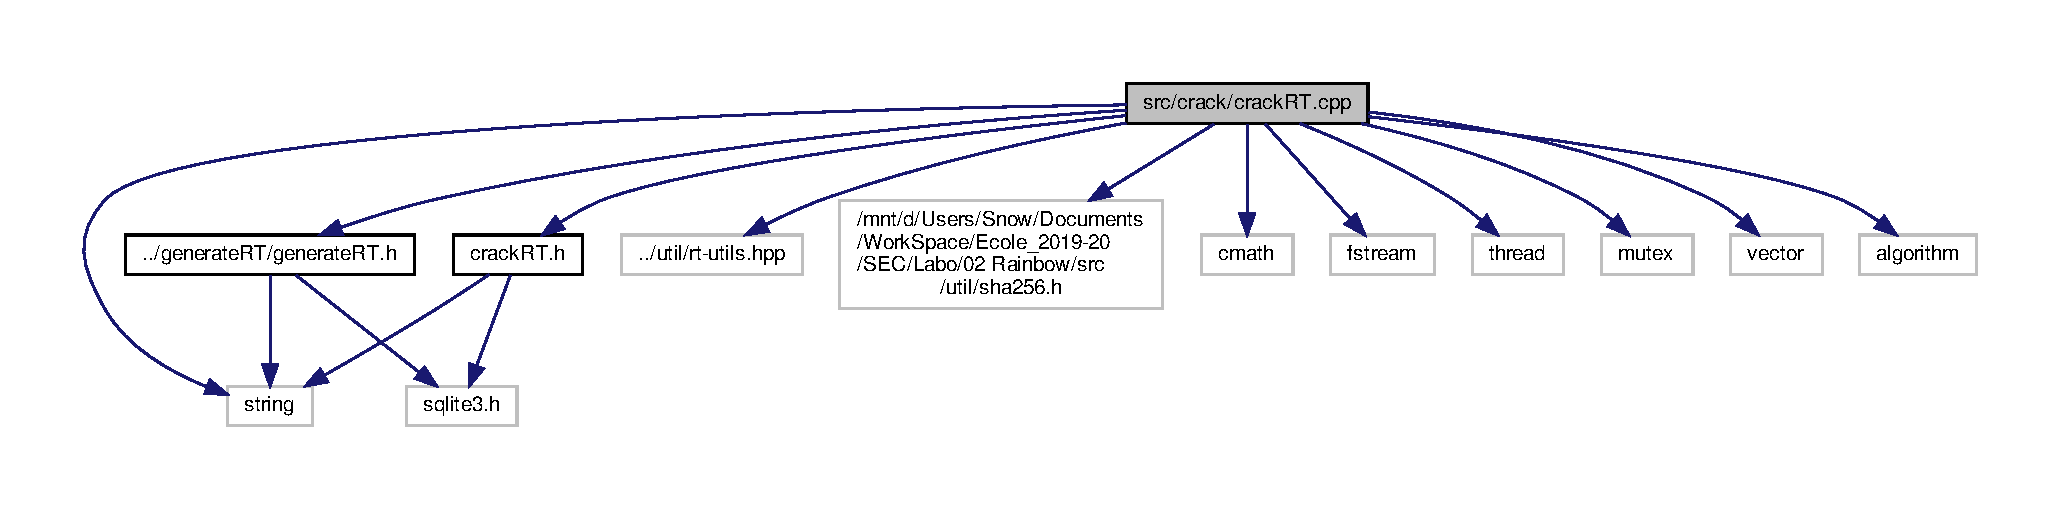
\includegraphics[width=350pt]{crackRT_8cpp__incl}
\end{center}
\end{figure}
\subsection*{Namespaces}
\begin{DoxyCompactItemize}
\item 
 \hyperlink{namespacebe_1_1esi_1_1secl_1_1pn}{be\+::esi\+::secl\+::pn}
\end{DoxyCompactItemize}
\subsection*{Functions}
\begin{DoxyCompactItemize}
\item 
void \hyperlink{namespacebe_1_1esi_1_1secl_1_1pn_aad832fb30fa4cc9e74d15d7129d0c929}{be\+::esi\+::secl\+::pn\+::crack} (const std\+::string \&hash\+File, sqlite3 $\ast$db, const std\+::string \&cracked\+Pwd\+File, const std\+::string \&cracked\+Hash\+File)
\begin{DoxyCompactList}\small\item\em Attempts to find passwords corresponding to the hashes given, at the hand of the tails. \end{DoxyCompactList}\item 
void \hyperlink{namespacebe_1_1esi_1_1secl_1_1pn_a5421a253f4c247695a0f26055ecc4dea}{be\+::esi\+::secl\+::pn\+::crack\+In\+Thread} (std\+::ifstream \&hashes\+Input, sqlite3 $\ast$db, std\+::ofstream \&cracked\+Pwd\+Output, std\+::ofstream \&cracked\+Hash\+Output)
\begin{DoxyCompactList}\small\item\em Crack function to call with a thread. \end{DoxyCompactList}\item 
std\+::string \hyperlink{namespacebe_1_1esi_1_1secl_1_1pn_a44dea6059d3689561497f5f03e09dac2}{be\+::esi\+::secl\+::pn\+::get\+Tail} (const std\+::string \&hash, sqlite3\+\_\+stmt $\ast$stmt\+Read\+Tail, int \&idx\+Reduction)
\begin{DoxyCompactList}\small\item\em Searches the tail of the hash and return it. \end{DoxyCompactList}\item 
std\+::string \hyperlink{namespacebe_1_1esi_1_1secl_1_1pn_a4f2bdcedf26f904e1e07776955d80d97}{be\+::esi\+::secl\+::pn\+::get\+Head} (sqlite3\+\_\+stmt $\ast$stmt\+Get\+Head, std\+::string tail)
\begin{DoxyCompactList}\small\item\em Get the head of a tail. \end{DoxyCompactList}\item 
std\+::string \hyperlink{namespacebe_1_1esi_1_1secl_1_1pn_ae68f13fff76cabc930b60594c300a168}{be\+::esi\+::secl\+::pn\+::find\+Pwd} (std\+::string head, int idx\+Reduction)
\begin{DoxyCompactList}\small\item\em Computes the password after idx\+Reduction reductions. \end{DoxyCompactList}\end{DoxyCompactItemize}
\subsection*{Variables}
\begin{DoxyCompactItemize}
\item 
std\+::mutex \hyperlink{namespacebe_1_1esi_1_1secl_1_1pn_ad1391e7f8a94f1b945665f76d1965070}{be\+::esi\+::secl\+::pn\+::mtx\+Read\+Head}
\begin{DoxyCompactList}\small\item\em Mutex to read the head file with concurency. \end{DoxyCompactList}\item 
std\+::mutex \hyperlink{namespacebe_1_1esi_1_1secl_1_1pn_a11fbbf54ca476439788d44d4d50512ab}{be\+::esi\+::secl\+::pn\+::mtx\+Print\+Cracked}
\begin{DoxyCompactList}\small\item\em Mutex to write cracked password and hashes with concurency. \end{DoxyCompactList}\item 
const unsigned \hyperlink{namespacebe_1_1esi_1_1secl_1_1pn_a0bd77d0531142c20d01ec002cd3c210a}{be\+::esi\+::secl\+::pn\+::\+N\+B\+\_\+\+T\+H\+R\+E\+A\+DS} = 10
\begin{DoxyCompactList}\small\item\em How many threads to run to crack. \end{DoxyCompactList}\end{DoxyCompactItemize}


\subsection{Detailed Description}
Declaration of functions of \hyperlink{crackRT_8h}{crack\+R\+T.\+h}. 


\hypertarget{crackRT_8h}{}\section{src/crack/crack\+RT.h File Reference}
\label{crackRT_8h}\index{src/crack/crack\+R\+T.\+h@{src/crack/crack\+R\+T.\+h}}


Declaration of functions of \hyperlink{crackRT_8h}{crack\+R\+T.\+h}.  


{\ttfamily \#include $<$string$>$}\newline
{\ttfamily \#include $<$sqlite3.\+h$>$}\newline
Include dependency graph for crack\+R\+T.\+h\+:
\nopagebreak
\begin{figure}[H]
\begin{center}
\leavevmode
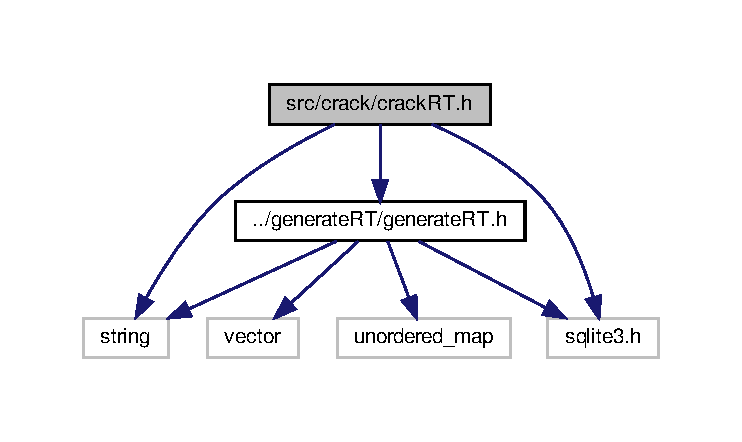
\includegraphics[width=193pt]{crackRT_8h__incl}
\end{center}
\end{figure}
This graph shows which files directly or indirectly include this file\+:
\nopagebreak
\begin{figure}[H]
\begin{center}
\leavevmode
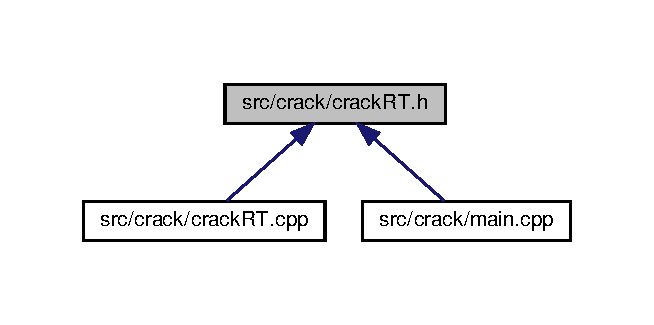
\includegraphics[width=314pt]{crackRT_8h__dep__incl}
\end{center}
\end{figure}
\subsection*{Namespaces}
\begin{DoxyCompactItemize}
\item 
 \hyperlink{namespacebe_1_1esi_1_1secl_1_1pn}{be\+::esi\+::secl\+::pn}
\end{DoxyCompactItemize}
\subsection*{Functions}
\begin{DoxyCompactItemize}
\item 
void \hyperlink{namespacebe_1_1esi_1_1secl_1_1pn_aad832fb30fa4cc9e74d15d7129d0c929}{be\+::esi\+::secl\+::pn\+::crack} (const std\+::string \&hash\+File, sqlite3 $\ast$db, const std\+::string \&cracked\+Pwd\+File, const std\+::string \&cracked\+Hash\+File)
\begin{DoxyCompactList}\small\item\em Attempts to find passwords corresponding to the hashes given, at the hand of the tails. \end{DoxyCompactList}\item 
void \hyperlink{namespacebe_1_1esi_1_1secl_1_1pn_a5421a253f4c247695a0f26055ecc4dea}{be\+::esi\+::secl\+::pn\+::crack\+In\+Thread} (std\+::ifstream \&hashes\+Input, sqlite3 $\ast$db, std\+::ofstream \&cracked\+Pwd\+Output, std\+::ofstream \&cracked\+Hash\+Output)
\begin{DoxyCompactList}\small\item\em Crack function to call with a thread. \end{DoxyCompactList}\item 
std\+::string \hyperlink{namespacebe_1_1esi_1_1secl_1_1pn_a44dea6059d3689561497f5f03e09dac2}{be\+::esi\+::secl\+::pn\+::get\+Tail} (const std\+::string \&hash, sqlite3\+\_\+stmt $\ast$stmt\+Read\+Tail, int \&idx\+Reduction)
\begin{DoxyCompactList}\small\item\em Searches the tail of the hash and return it. \end{DoxyCompactList}\item 
std\+::string \hyperlink{namespacebe_1_1esi_1_1secl_1_1pn_a4f2bdcedf26f904e1e07776955d80d97}{be\+::esi\+::secl\+::pn\+::get\+Head} (sqlite3\+\_\+stmt $\ast$stmt\+Get\+Head, std\+::string tail)
\begin{DoxyCompactList}\small\item\em Get the head of a tail. \end{DoxyCompactList}\item 
std\+::string \hyperlink{namespacebe_1_1esi_1_1secl_1_1pn_ae68f13fff76cabc930b60594c300a168}{be\+::esi\+::secl\+::pn\+::find\+Pwd} (std\+::string head, int idx\+Reduction)
\begin{DoxyCompactList}\small\item\em Computes the password after idx\+Reduction reductions. \end{DoxyCompactList}\end{DoxyCompactItemize}
\subsection*{Variables}
\begin{DoxyCompactItemize}
\item 
const char $\ast$ \hyperlink{namespacebe_1_1esi_1_1secl_1_1pn_a878205e4dbef8040fb12f6afb8717fa9}{be\+::esi\+::secl\+::pn\+::\+S\+E\+L\+E\+C\+T\+\_\+\+T\+A\+IL} = \char`\"{}S\+E\+L\+E\+CT tail F\+R\+OM R\+A\+I\+N\+B\+O\+W\+\_\+\+T\+A\+B\+LE W\+H\+E\+RE tail = ?;\char`\"{}
\begin{DoxyCompactList}\small\item\em Select a tail. \end{DoxyCompactList}\item 
const char $\ast$ \hyperlink{namespacebe_1_1esi_1_1secl_1_1pn_a90db4018123c098c9cd9205b69c1d2e5}{be\+::esi\+::secl\+::pn\+::\+S\+E\+L\+E\+C\+T\+\_\+\+H\+E\+AD} = \char`\"{}S\+E\+L\+E\+CT head F\+R\+OM R\+A\+I\+N\+B\+O\+W\+\_\+\+T\+A\+B\+LE W\+H\+E\+RE tail = ?;\char`\"{}
\begin{DoxyCompactList}\small\item\em Select the head of the tail. \end{DoxyCompactList}\end{DoxyCompactItemize}


\subsection{Detailed Description}
Declaration of functions of \hyperlink{crackRT_8h}{crack\+R\+T.\+h}. 


\hypertarget{crack_2main_8cpp}{}\section{src/crack/main.cpp File Reference}
\label{crack_2main_8cpp}\index{src/crack/main.\+cpp@{src/crack/main.\+cpp}}
{\ttfamily \#include \char`\"{}crack\+R\+T.\+h\char`\"{}}\newline
{\ttfamily \#include \char`\"{}../util/passwd-\/utils.\+hpp\char`\"{}}\newline
{\ttfamily \#include $<$string$>$}\newline
{\ttfamily \#include $<$iostream$>$}\newline
{\ttfamily \#include $<$sqlite3.\+h$>$}\newline
Include dependency graph for main.\+cpp\+:\nopagebreak
\begin{figure}[H]
\begin{center}
\leavevmode
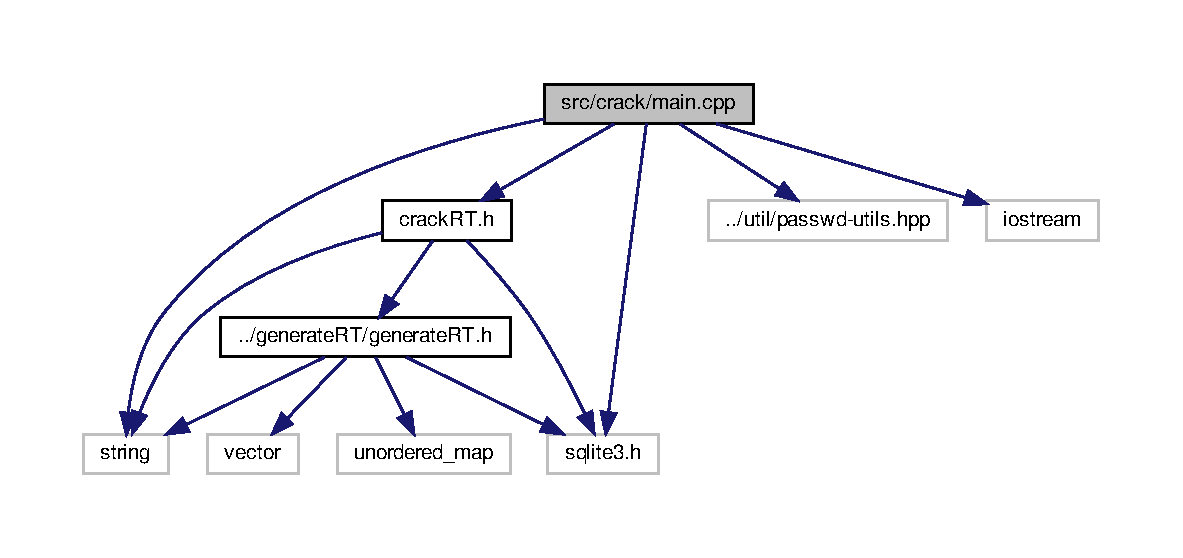
\includegraphics[width=350pt]{crack_2main_8cpp__incl}
\end{center}
\end{figure}
\subsection*{Functions}
\begin{DoxyCompactItemize}
\item 
const std\+::string \hyperlink{crack_2main_8cpp_a4ec938e7b7ae40c2ec0db22f3968e4ec}{P\+W\+D\+\_\+\+F\+I\+LE} (\char`\"{}rsc/pwd\+To\+Crack.\+txt\char`\"{})
\begin{DoxyCompactList}\small\item\em The file which will contain some passwords. \end{DoxyCompactList}\item 
const std\+::string \hyperlink{crack_2main_8cpp_ab676e49dba7ead58917e5080eb754415}{H\+A\+S\+H\+\_\+\+F\+I\+LE} (\char`\"{}rsc/hash\+To\+Crack.\+txt\char`\"{})
\begin{DoxyCompactList}\small\item\em The file which will contain the passwords hashes to crack. \end{DoxyCompactList}\item 
const std\+::string \hyperlink{crack_2main_8cpp_aacc8f3b1b0f003879782a222a831aebb}{C\+R\+A\+C\+K\+E\+D\+\_\+\+P\+W\+D\+\_\+\+F\+I\+LE} (\char`\"{}rsc/cracked\+Pwd.\+txt\char`\"{})
\begin{DoxyCompactList}\small\item\em The file which will contain the cracked passwords. \end{DoxyCompactList}\item 
const std\+::string \hyperlink{crack_2main_8cpp_a6c3c6345561be266b0c9a7e40a477d45}{C\+R\+A\+C\+K\+E\+D\+\_\+\+H\+A\+S\+H\+\_\+\+F\+I\+LE} (\char`\"{}rsc/cracked\+Hash.\+txt\char`\"{})
\begin{DoxyCompactList}\small\item\em The file which will contain the cracked passwords hashes. \end{DoxyCompactList}\item 
int \hyperlink{crack_2main_8cpp_ae66f6b31b5ad750f1fe042a706a4e3d4}{main} ()
\begin{DoxyCompactList}\small\item\em Entry for the crack. \end{DoxyCompactList}\end{DoxyCompactItemize}


\subsection{Function Documentation}
\mbox{\Hypertarget{crack_2main_8cpp_a6c3c6345561be266b0c9a7e40a477d45}\label{crack_2main_8cpp_a6c3c6345561be266b0c9a7e40a477d45}} 
\index{crack/main.\+cpp@{crack/main.\+cpp}!C\+R\+A\+C\+K\+E\+D\+\_\+\+H\+A\+S\+H\+\_\+\+F\+I\+LE@{C\+R\+A\+C\+K\+E\+D\+\_\+\+H\+A\+S\+H\+\_\+\+F\+I\+LE}}
\index{C\+R\+A\+C\+K\+E\+D\+\_\+\+H\+A\+S\+H\+\_\+\+F\+I\+LE@{C\+R\+A\+C\+K\+E\+D\+\_\+\+H\+A\+S\+H\+\_\+\+F\+I\+LE}!crack/main.\+cpp@{crack/main.\+cpp}}
\subsubsection{\texorpdfstring{C\+R\+A\+C\+K\+E\+D\+\_\+\+H\+A\+S\+H\+\_\+\+F\+I\+L\+E()}{CRACKED\_HASH\_FILE()}}
{\footnotesize\ttfamily const std\+::string C\+R\+A\+C\+K\+E\+D\+\_\+\+H\+A\+S\+H\+\_\+\+F\+I\+LE (\begin{DoxyParamCaption}\item[{\char`\"{}rsc/cracked\+Hash.\+txt\char`\"{}}]{ }\end{DoxyParamCaption})}



The file which will contain the cracked passwords hashes. 

\mbox{\Hypertarget{crack_2main_8cpp_aacc8f3b1b0f003879782a222a831aebb}\label{crack_2main_8cpp_aacc8f3b1b0f003879782a222a831aebb}} 
\index{crack/main.\+cpp@{crack/main.\+cpp}!C\+R\+A\+C\+K\+E\+D\+\_\+\+P\+W\+D\+\_\+\+F\+I\+LE@{C\+R\+A\+C\+K\+E\+D\+\_\+\+P\+W\+D\+\_\+\+F\+I\+LE}}
\index{C\+R\+A\+C\+K\+E\+D\+\_\+\+P\+W\+D\+\_\+\+F\+I\+LE@{C\+R\+A\+C\+K\+E\+D\+\_\+\+P\+W\+D\+\_\+\+F\+I\+LE}!crack/main.\+cpp@{crack/main.\+cpp}}
\subsubsection{\texorpdfstring{C\+R\+A\+C\+K\+E\+D\+\_\+\+P\+W\+D\+\_\+\+F\+I\+L\+E()}{CRACKED\_PWD\_FILE()}}
{\footnotesize\ttfamily const std\+::string C\+R\+A\+C\+K\+E\+D\+\_\+\+P\+W\+D\+\_\+\+F\+I\+LE (\begin{DoxyParamCaption}\item[{\char`\"{}rsc/cracked\+Pwd.\+txt\char`\"{}}]{ }\end{DoxyParamCaption})}



The file which will contain the cracked passwords. 

\mbox{\Hypertarget{crack_2main_8cpp_ab676e49dba7ead58917e5080eb754415}\label{crack_2main_8cpp_ab676e49dba7ead58917e5080eb754415}} 
\index{crack/main.\+cpp@{crack/main.\+cpp}!H\+A\+S\+H\+\_\+\+F\+I\+LE@{H\+A\+S\+H\+\_\+\+F\+I\+LE}}
\index{H\+A\+S\+H\+\_\+\+F\+I\+LE@{H\+A\+S\+H\+\_\+\+F\+I\+LE}!crack/main.\+cpp@{crack/main.\+cpp}}
\subsubsection{\texorpdfstring{H\+A\+S\+H\+\_\+\+F\+I\+L\+E()}{HASH\_FILE()}}
{\footnotesize\ttfamily const std\+::string H\+A\+S\+H\+\_\+\+F\+I\+LE (\begin{DoxyParamCaption}\item[{\char`\"{}rsc/hash\+To\+Crack.\+txt\char`\"{}}]{ }\end{DoxyParamCaption})}



The file which will contain the passwords hashes to crack. 

\mbox{\Hypertarget{crack_2main_8cpp_ae66f6b31b5ad750f1fe042a706a4e3d4}\label{crack_2main_8cpp_ae66f6b31b5ad750f1fe042a706a4e3d4}} 
\index{crack/main.\+cpp@{crack/main.\+cpp}!main@{main}}
\index{main@{main}!crack/main.\+cpp@{crack/main.\+cpp}}
\subsubsection{\texorpdfstring{main()}{main()}}
{\footnotesize\ttfamily int main (\begin{DoxyParamCaption}{ }\end{DoxyParamCaption})}



Entry for the crack. 

It will generate some passwords (+ hashes), and crack them with the rainbow table. The cracked passwords and hashes are put into a new file. This is needed to keep the passwords and hashes sorted, due to the use of threads. \mbox{\Hypertarget{crack_2main_8cpp_a4ec938e7b7ae40c2ec0db22f3968e4ec}\label{crack_2main_8cpp_a4ec938e7b7ae40c2ec0db22f3968e4ec}} 
\index{crack/main.\+cpp@{crack/main.\+cpp}!P\+W\+D\+\_\+\+F\+I\+LE@{P\+W\+D\+\_\+\+F\+I\+LE}}
\index{P\+W\+D\+\_\+\+F\+I\+LE@{P\+W\+D\+\_\+\+F\+I\+LE}!crack/main.\+cpp@{crack/main.\+cpp}}
\subsubsection{\texorpdfstring{P\+W\+D\+\_\+\+F\+I\+L\+E()}{PWD\_FILE()}}
{\footnotesize\ttfamily const std\+::string P\+W\+D\+\_\+\+F\+I\+LE (\begin{DoxyParamCaption}\item[{\char`\"{}rsc/pwd\+To\+Crack.\+txt\char`\"{}}]{ }\end{DoxyParamCaption})}



The file which will contain some passwords. 

This file is not necessary to crack 
\hypertarget{generateRT_2main_8cpp}{}\section{src/generate\+R\+T/main.cpp File Reference}
\label{generateRT_2main_8cpp}\index{src/generate\+R\+T/main.\+cpp@{src/generate\+R\+T/main.\+cpp}}
{\ttfamily \#include \char`\"{}generate\+R\+T.\+h\char`\"{}}\newline
{\ttfamily \#include $<$iostream$>$}\newline
{\ttfamily \#include $<$string$>$}\newline
{\ttfamily \#include $<$sqlite3.\+h$>$}\newline
{\ttfamily \#include $<$sstream$>$}\newline
{\ttfamily \#include $<$fstream$>$}\newline
{\ttfamily \#include $<$filesystem$>$}\newline
{\ttfamily \#include \char`\"{}../util/rt-\/utils.\+hpp\char`\"{}}\newline
Include dependency graph for main.\+cpp\+:\nopagebreak
\begin{figure}[H]
\begin{center}
\leavevmode
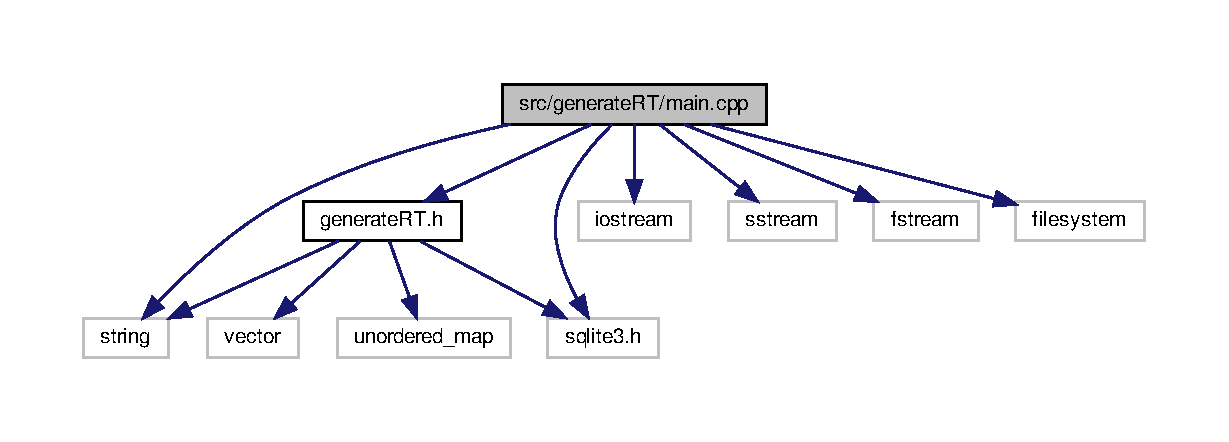
\includegraphics[width=350pt]{generateRT_2main_8cpp__incl}
\end{center}
\end{figure}
\subsection*{Functions}
\begin{DoxyCompactItemize}
\item 
int \hyperlink{generateRT_2main_8cpp_a0ddf1224851353fc92bfbff6f499fa97}{main} (int argc, char $\ast$argv\mbox{[}$\,$\mbox{]})
\begin{DoxyCompactList}\small\item\em Entry point to generate the Rainbow Table. \end{DoxyCompactList}\end{DoxyCompactItemize}
\subsection*{Variables}
\begin{DoxyCompactItemize}
\item 
unsigned long long \hyperlink{generateRT_2main_8cpp_afb61832834f9080d06074c378682025d}{S\+I\+Z\+E\+\_\+\+DB} = 12\+U\+L\+L $\ast$ 1024\+U\+L\+L $\ast$ 1024\+U\+L\+L $\ast$ 1024\+U\+LL
\begin{DoxyCompactList}\small\item\em The size of the file for the DB. \end{DoxyCompactList}\end{DoxyCompactItemize}


\subsection{Function Documentation}
\mbox{\Hypertarget{generateRT_2main_8cpp_a0ddf1224851353fc92bfbff6f499fa97}\label{generateRT_2main_8cpp_a0ddf1224851353fc92bfbff6f499fa97}} 
\index{generate\+R\+T/main.\+cpp@{generate\+R\+T/main.\+cpp}!main@{main}}
\index{main@{main}!generate\+R\+T/main.\+cpp@{generate\+R\+T/main.\+cpp}}
\subsubsection{\texorpdfstring{main()}{main()}}
{\footnotesize\ttfamily int main (\begin{DoxyParamCaption}\item[{int}]{argc,  }\item[{char $\ast$}]{argv\mbox{[}$\,$\mbox{]} }\end{DoxyParamCaption})}



Entry point to generate the Rainbow Table. 

It will create and open a sqlite DB, and set it up with a configuration that maximizes speed. Note that with some configuration, the database can be corrupted in the event of a crash or power outage. After that, it will generate the RT with default (ne param) or user values (first param is the number of head to create, second is the number of reduce to apply). 
\begin{DoxyParams}{Parameters}
{\em argc} & The number of params \\
\hline
{\em argv} & The params. Can be empty. If not empty, param at position 1 and 2 must be numericals values. The first is the number of head to create, the second the number of reduce to apply on the head to get the tail. If the value is not correct, behavior is undetermined. \\
\hline
\end{DoxyParams}


\subsection{Variable Documentation}
\mbox{\Hypertarget{generateRT_2main_8cpp_afb61832834f9080d06074c378682025d}\label{generateRT_2main_8cpp_afb61832834f9080d06074c378682025d}} 
\index{generate\+R\+T/main.\+cpp@{generate\+R\+T/main.\+cpp}!S\+I\+Z\+E\+\_\+\+DB@{S\+I\+Z\+E\+\_\+\+DB}}
\index{S\+I\+Z\+E\+\_\+\+DB@{S\+I\+Z\+E\+\_\+\+DB}!generate\+R\+T/main.\+cpp@{generate\+R\+T/main.\+cpp}}
\subsubsection{\texorpdfstring{S\+I\+Z\+E\+\_\+\+DB}{SIZE\_DB}}
{\footnotesize\ttfamily unsigned long long S\+I\+Z\+E\+\_\+\+DB = 12\+U\+L\+L $\ast$ 1024\+U\+L\+L $\ast$ 1024\+U\+L\+L $\ast$ 1024\+U\+LL}



The size of the file for the DB. 


\hypertarget{generateRT_8cpp}{}\section{src/generate\+R\+T/generate\+RT.cpp File Reference}
\label{generateRT_8cpp}\index{src/generate\+R\+T/generate\+R\+T.\+cpp@{src/generate\+R\+T/generate\+R\+T.\+cpp}}


Definition of function of \hyperlink{generateRT_8h}{generate\+R\+T.\+h}.  


{\ttfamily \#include \char`\"{}../util/passwd-\/utils.\+hpp\char`\"{}}\newline
{\ttfamily \#include \char`\"{}../util/rt-\/utils.\+hpp\char`\"{}}\newline
{\ttfamily \#include \char`\"{}generate\+R\+T.\+h\char`\"{}}\newline
{\ttfamily \#include $<$fstream$>$}\newline
{\ttfamily \#include $<$algorithm$>$}\newline
{\ttfamily \#include $<$thread$>$}\newline
Include dependency graph for generate\+R\+T.\+cpp\+:
\nopagebreak
\begin{figure}[H]
\begin{center}
\leavevmode
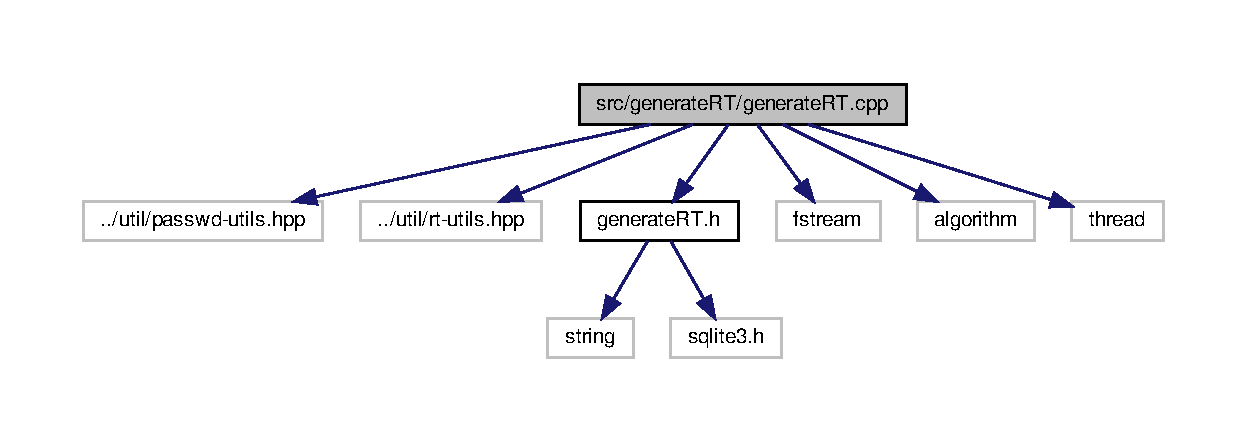
\includegraphics[width=350pt]{generateRT_8cpp__incl}
\end{center}
\end{figure}
\subsection*{Namespaces}
\begin{DoxyCompactItemize}
\item 
 \hyperlink{namespacebe_1_1esi_1_1secl_1_1pn}{be\+::esi\+::secl\+::pn}
\end{DoxyCompactItemize}
\subsection*{Functions}
\begin{DoxyCompactItemize}
\item 
void \hyperlink{namespacebe_1_1esi_1_1secl_1_1pn_af8b773cad93b0eb78b89f69721e4bb1d}{be\+::esi\+::secl\+::pn\+::generate\+RT} (sqlite3 $\ast$db, unsigned nb\+Head=N\+B\+\_\+\+H\+E\+AD, int nb\+Reduce=N\+B\+\_\+\+R\+E\+D\+U\+CE)
\begin{DoxyCompactList}\small\item\em Generate the head and the tails of the RT, and write them into the DB. \end{DoxyCompactList}\item 
void \hyperlink{namespacebe_1_1esi_1_1secl_1_1pn_aaf5216f5718720c15b5925f7e8a94d10}{be\+::esi\+::secl\+::pn\+::generate\+R\+T\+In\+Thread} (sqlite3 $\ast$db, unsigned nb\+Head, int nb\+Reduce)
\begin{DoxyCompactList}\small\item\em Generate the head and the tails of the RT, and write them into the DB. \end{DoxyCompactList}\end{DoxyCompactItemize}
\subsection*{Variables}
\begin{DoxyCompactItemize}
\item 
const unsigned \hyperlink{namespacebe_1_1esi_1_1secl_1_1pn_a6b1322df9a3137fe3dff27602a0dd390}{be\+::esi\+::secl\+::pn\+::\+N\+B\+\_\+\+T\+H\+R\+E\+A\+D\+S\+\_\+\+G\+E\+N\+E\+R\+A\+TE} = 10
\begin{DoxyCompactList}\small\item\em Number of thread to create to generate the RT. \end{DoxyCompactList}\end{DoxyCompactItemize}


\subsection{Detailed Description}
Definition of function of \hyperlink{generateRT_8h}{generate\+R\+T.\+h}. 


\hypertarget{generateRT_8h}{}\section{src/generate\+R\+T/generate\+RT.h File Reference}
\label{generateRT_8h}\index{src/generate\+R\+T/generate\+R\+T.\+h@{src/generate\+R\+T/generate\+R\+T.\+h}}


Declaration of functions for \hyperlink{generateRT_8cpp}{generate\+R\+T.\+cpp}.  


{\ttfamily \#include $<$string$>$}\newline
{\ttfamily \#include $<$sqlite3.\+h$>$}\newline
Include dependency graph for generate\+R\+T.\+h\+:
\nopagebreak
\begin{figure}[H]
\begin{center}
\leavevmode
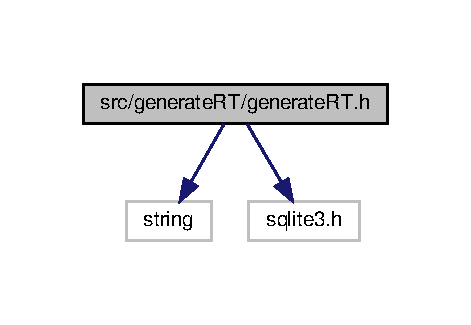
\includegraphics[width=226pt]{generateRT_8h__incl}
\end{center}
\end{figure}
This graph shows which files directly or indirectly include this file\+:
\nopagebreak
\begin{figure}[H]
\begin{center}
\leavevmode
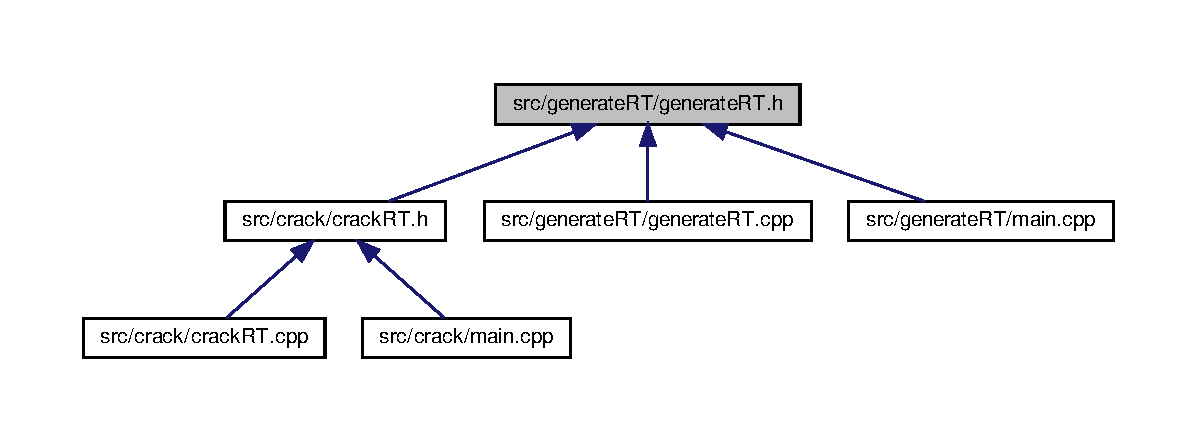
\includegraphics[width=350pt]{generateRT_8h__dep__incl}
\end{center}
\end{figure}
\subsection*{Namespaces}
\begin{DoxyCompactItemize}
\item 
 \hyperlink{namespacebe_1_1esi_1_1secl_1_1pn}{be\+::esi\+::secl\+::pn}
\end{DoxyCompactItemize}
\subsection*{Functions}
\begin{DoxyCompactItemize}
\item 
const std\+::string \hyperlink{namespacebe_1_1esi_1_1secl_1_1pn_a6b6903f68a7fbdcd8e705dc2b9c28c03}{be\+::esi\+::secl\+::pn\+::\+D\+B\+\_\+\+N\+A\+ME} (\char`\"{}rsc/rt\+\_\+6\+\_\+2\+\_\+1000000\+\_\+1000.\+sqlite\char`\"{})
\begin{DoxyCompactList}\small\item\em The relative path to the DB. \end{DoxyCompactList}\item 
void \hyperlink{namespacebe_1_1esi_1_1secl_1_1pn_af8b773cad93b0eb78b89f69721e4bb1d}{be\+::esi\+::secl\+::pn\+::generate\+RT} (sqlite3 $\ast$db, unsigned nb\+Head=N\+B\+\_\+\+H\+E\+AD, int nb\+Reduce=N\+B\+\_\+\+R\+E\+D\+U\+CE)
\begin{DoxyCompactList}\small\item\em Generate the head and the tails of the RT, and write them into the DB. \end{DoxyCompactList}\item 
void \hyperlink{namespacebe_1_1esi_1_1secl_1_1pn_aaf5216f5718720c15b5925f7e8a94d10}{be\+::esi\+::secl\+::pn\+::generate\+R\+T\+In\+Thread} (sqlite3 $\ast$db, unsigned nb\+Head, int nb\+Reduce)
\begin{DoxyCompactList}\small\item\em Generate the head and the tails of the RT, and write them into the DB. \end{DoxyCompactList}\end{DoxyCompactItemize}
\subsection*{Variables}
\begin{DoxyCompactItemize}
\item 
const unsigned \hyperlink{namespacebe_1_1esi_1_1secl_1_1pn_a3f7aaccb1bf4e47f92d72bf9b2471328}{be\+::esi\+::secl\+::pn\+::\+N\+B\+\_\+\+H\+E\+AD} = 500000000
\begin{DoxyCompactList}\small\item\em How many password we generate for the RT. \end{DoxyCompactList}\item 
const int \hyperlink{namespacebe_1_1esi_1_1secl_1_1pn_a9434f9e96778e243fcb677633df38598}{be\+::esi\+::secl\+::pn\+::\+N\+B\+\_\+\+R\+E\+D\+U\+CE} = 160
\begin{DoxyCompactList}\small\item\em How many reduce function we use before getting the tail. \end{DoxyCompactList}\item 
const unsigned \hyperlink{namespacebe_1_1esi_1_1secl_1_1pn_ac4d6305d2a5baed196042f8a30533620}{be\+::esi\+::secl\+::pn\+::\+M\+I\+N\+\_\+\+P\+W\+D\+\_\+\+S\+I\+ZE} = 6
\begin{DoxyCompactList}\small\item\em The minimal password size. \end{DoxyCompactList}\item 
const unsigned \hyperlink{namespacebe_1_1esi_1_1secl_1_1pn_a2e3241ac36dabdb668b68028e097dded}{be\+::esi\+::secl\+::pn\+::\+M\+A\+X\+\_\+\+P\+W\+D\+\_\+\+S\+I\+ZE} = 6
\begin{DoxyCompactList}\small\item\em The maximal password size. \end{DoxyCompactList}\item 
const char $\ast$ \hyperlink{namespacebe_1_1esi_1_1secl_1_1pn_a6dae14cb83aa871e50c9aaea7f776055}{be\+::esi\+::secl\+::pn\+::\+D\+R\+O\+P\+\_\+\+RT} = \char`\"{}D\+R\+OP T\+A\+B\+LE IF E\+X\+I\+S\+TS R\+A\+I\+N\+B\+O\+W\+\_\+\+T\+A\+B\+LE;\char`\"{}
\item 
const char $\ast$ \hyperlink{namespacebe_1_1esi_1_1secl_1_1pn_ab39f379fcf2d9342096df70dcf998d32}{be\+::esi\+::secl\+::pn\+::\+C\+R\+E\+A\+T\+E\+\_\+\+RT} = \char`\"{}C\+R\+E\+A\+TE T\+A\+B\+LE R\+A\+I\+N\+B\+O\+W\+\_\+\+T\+A\+B\+LE (head C\+H\+AR(8) P\+R\+I\+M\+A\+RY K\+EY, tail C\+H\+AR(8) N\+OT N\+U\+LL U\+N\+I\+Q\+UE);\char`\"{}
\item 
const char $\ast$ \hyperlink{namespacebe_1_1esi_1_1secl_1_1pn_a93b0970fb08c37d478307bfadfb3b775}{be\+::esi\+::secl\+::pn\+::\+I\+N\+S\+E\+R\+T\+\_\+\+RT} = \char`\"{}I\+N\+S\+E\+RT OR I\+G\+N\+O\+RE I\+N\+TO R\+A\+I\+N\+B\+O\+W\+\_\+\+T\+A\+B\+LE (head, tail) V\+A\+L\+U\+ES (?, ?);\char`\"{}
\end{DoxyCompactItemize}


\subsection{Detailed Description}
Declaration of functions for \hyperlink{generateRT_8cpp}{generate\+R\+T.\+cpp}. 


%--- End generated contents ---

% Index
\backmatter
\newpage
\phantomsection
\clearemptydoublepage
\addcontentsline{toc}{chapter}{Index}
\printindex

\end{document}
